\subsubsection{Función de activación}\label{activationfunction}

Lo anterior, se puede comprobar matemáticamente que el efecto de sumar muchas operaciones de regresión lineal equivale a una única regresión lineal. Esto se demuestra en la sección \ref{feedforward}. El perceptrón que se ha creado puede colapsar hasta ser equivalente a tener una única neurona. Para evitar esto, debemos calcular valores que no den como resultado una función lineal(una línea recta en dos dimensiones), necesitamos que cada una de estas neuronas aplique alguna función para realizar algún tipo de manipulación no lineal que distorsione sus valores de salida y para ello se usan las funciones de activación \cite{nielsen}.
\newline

A modo de ejemplo, se mostrará con un ejemplo con un modelo con solo funciones lineales comparado con un modelo que usa funciones no lineales. Para ello, se expone el siguiente ejemplo: se quiere crear un modelo de regresión que trate de predecir el valor de una función seno. Al ser el seno una función no lineal, se necesitará de funciones no lineales para resolver el problema.

\begin{equation}
    y = \sin(x)
\end{equation}

También se mostrará código para ir introduciendo el funcionamiento de las librerías que se usan popularmente en mundo del \textit{machine learnig}. Como se explica en la sección \ref{used_libs}, en este trabajo se han usado \verb|keras|(redes neuronales), \verb|numpy|(vectores y matrices) y \verb|matplotlib|(representar funciones) entre otras. 
\newline

Como se explica en la sección de entrenamiento(sección \ref{training}), se necesita un dataset para que la red se pueda entrenar. El dataset se creará de la siguiente forma:


\begin{minted}[fontsize=\footnotesize]{python}
# real sen data
x = np.linspace(0, 2*np.pi, 1000)
y = np.sin(x)

# some noise is added to the real dataset to make it 
# look like a real world data set
noise = 0.1
noisex = x + np.random.normal(-noise, noise, 1000)
noisey = y + np.random.normal(-noise, noise, 1000)
\end{minted}

Gráficamente quedaría una serie de puntos esparcidos alrededor de la función seno como es de esperar:
\begin{figure}[H]
    \centering
    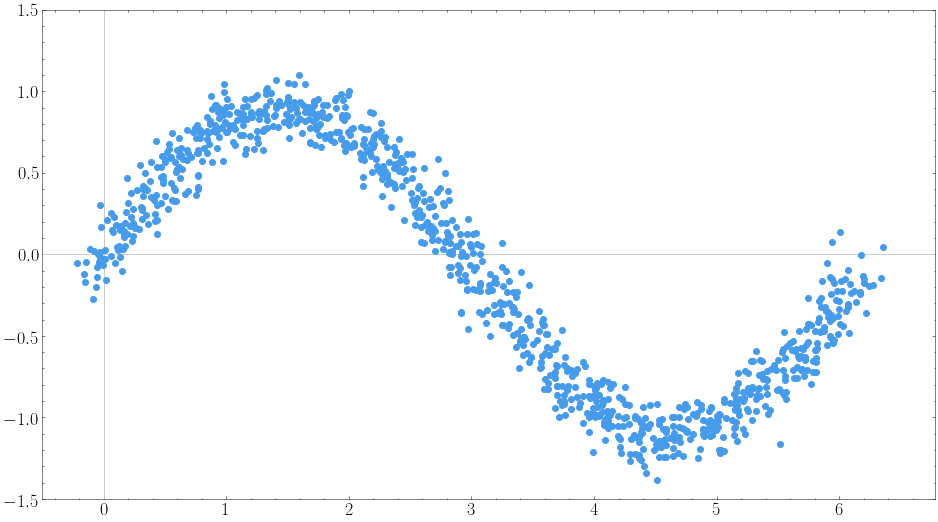
\includegraphics[width=11cm]{images/state-of-art/activation-functions/sin.png}
    \caption{Dataset emulando una función seno}
    \label{fig:basicneuron}
\end{figure}

Se crearán dos modelos, es decir, dos redes con arquitecturas distintas: Un modelo con funciones de activación lineales(\verb|linear_model|) y otro con funciones de activación no lineales(\verb|relu_model|).
\newline

El primer modelo viene definido de la siguiente forma:

\begin{minted}[fontsize=\footnotesize]{python}
linear_model = Sequential()
linear_model.add(Dense(32, activation='linear'))
linear_model.add(Dense(32, activation='linear'))
linear_model.add(Dense(1))
\end{minted}

Lo que se hace en ese código es crear la arquitectura de la red. Será una red con tres capas densas. Las dos primeras capas son las capas ocultas del modelo y se indica que se quieren 32 neuronas en cada capa con la función de activación \verb|linear|. La última capa simplemente es para que el modelo solo devuelva un único valor.
\newline

La otra red usará una función no lineal de activación \acrshort{relu}, explicada posteriormente. EL código para la arquitectura de esta red es la siguiente:
\begin{minted}[fontsize=\footnotesize]{python}
relu_model = Sequential()
relu_model.add(Dense(32, activation='relu'))
relu_model.add(Dense(32, activation='relu'))
relu_model.add(Dense(1))
\end{minted}

Posteriormente se "compila" el modelo. En este paso, se indicará a \textit{keras} que se parámetros tanto obligatorios como opcionales se quieren para red. Estos parámetros serán explicados en próximas secciones. Justo después se entrena a los modelos.
\begin{minted}[fontsize=\footnotesize]{python}
# Compile linear model
linear_model.compile(loss='mean_squared_error', 
                     optimizer='adam')
# Train linear model
linear_model.fit(noisex, noisey, epochs=100, verbose=0)

# Compile ReLU model
relu_model.compile(loss='mean_squared_error',
                   optimizer='adam')
# Train ReLU model
relu_model.fit(noisex, noisey, epochs=100, verbose=0)
\end{minted}

Para realizar una predición con estos modelos simplemente se puede usar la función \verb|predict()| del modelo:
\begin{minted}[fontsize=\footnotesize]{python}
predicted_by_linear = linear_model.predict(x)
predicted_by_relu = relu_model.predict(x)

# Plot predictions
plt.plot(x, predicted_by_linear)
plt.plot(x, predicted_by_relu)
\end{minted}

\begin{figure}[H]
    \centering
    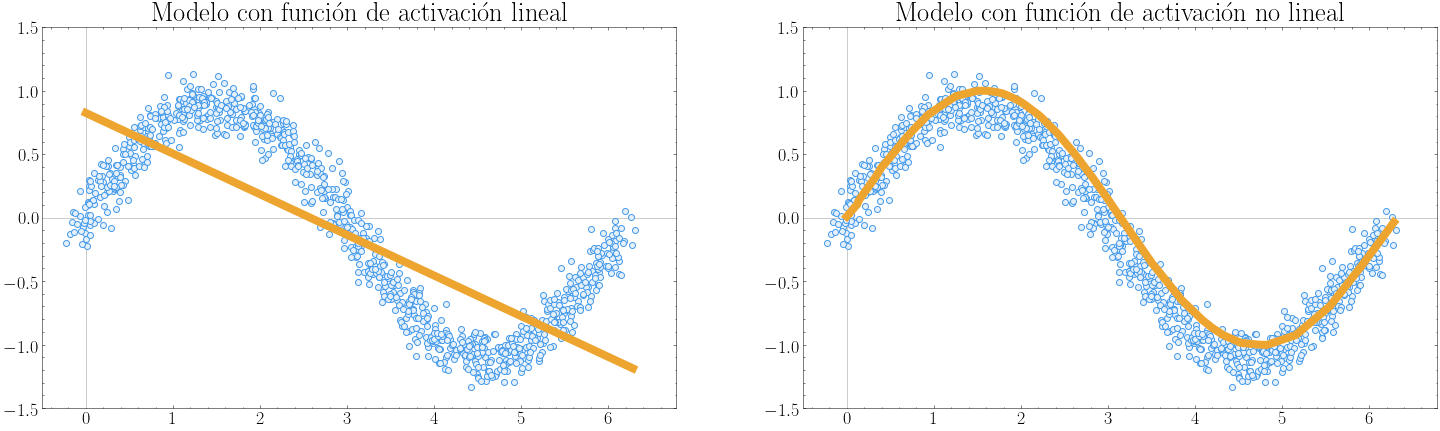
\includegraphics[width=15cm]{images/state-of-art/activation-functions/sin_activation_function.png}
    \caption{Comparativa de funciones de activación lineal y no lineal}
    \label{fig:basicneuron}
\end{figure}

Como se puede observar, el modelo que usa una función de activación lineal se reduce a una única recta mientras que el modelo que usa una función de activación no lineal se adapta correctamente.
\newline

En resumen, la función de activación es una función que se aplica al resultado de la suma ponderada de los valores de entrada, es decir, a $z$. El objetivo es que distorsione el resultado de la neurona añadiéndole deformaciones no lineales para que así se pueda encadenar de forma efectiva la computación de varias neuronas. Se representará esta función de activación de la siguiente forma:

\begin{equation}
    a(z) = a(w \cdot x + b)
    \label{eqn:activationfunctionbasic}
\end{equation}

Actualizando la imagen que se ha usado antes para definir un perceptrón, quedaría tal que:
\begin{figure}[H]
    \centering
    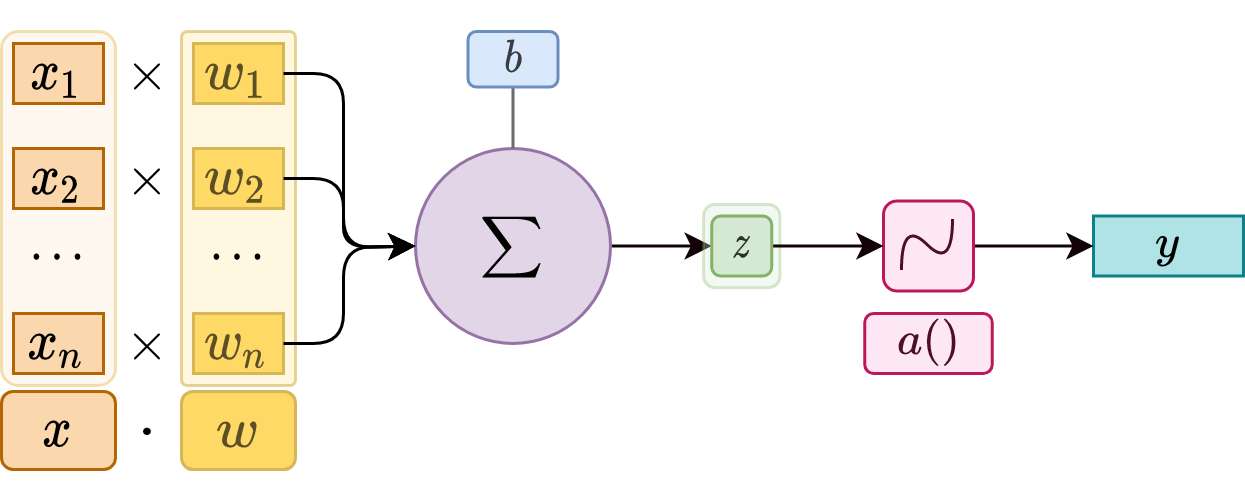
\includegraphics[width=10cm]{images/state-of-art/activation-functions/activation_representation.png}
    \caption{Representación de funcionamiento de una neurona}
    \label{fig:basicneuron}
\end{figure}

Existen varios tipos de función de activación, estas son las más usadas:

\begin{itemize}
\item Lineal: Es simplemente la ecuación de una recta y por lo tanto una función lineal. Normalmente se utiliza en la última capa en un modelo de regresión, es decir, un modelo que realiza una tarea de regresión y no una tarea de clasificación.
\begin{eqnarray}
  a(z) & = & z \\
  a'(z) & = & 1 
\end{eqnarray}

\item Escalonada (\textit{step} en inglés): El objetivo de la función es convertir los valores a $0$ o a $1$ en función de $b$. El propósito de esta función de activación es imitar una neurona que "se activa" o "no se activa" basándose en la información de entrada. Tradicionalmente, esta función se usaba en las redes de perceptrones y de hecho, es la usada en la ecuación \ref{eqn:perceptroncomplex}. La ecuación es la siguiente:

\begin{eqnarray}
  a(z) & = & \left\{ \begin{array}{ll}
      0 & \mbox{si } z \leq 0 \\
      1 & \mbox{si } z > 0
      \end{array} \right. \\
     \newline
  a'(z) & = & 0 
\end{eqnarray}


\item \acrfull{relu}: Es una función lineal cuando es positiva y constante a 0 cuando el valor es negativo. Es muy usada porque es una función no lineal y parecida a la función lineal, por lo que es rápido de computar.

\begin{eqnarray}
    a(z) & = & max(0,z) \\
  a'(z) & = & \left\{ \begin{array}{ll}
      0 & \mbox{si } z \leq 0   \\
      1 & \mbox{si } z > 0 
      \end{array} \right.
\end{eqnarray}

Existe una variante de esta función de activación (conocida como \textit{leaky}). En esta variante, se cambia la inclinación a un valor $s$ de la parte negativa respecto al eje de abscisas. 
\begin{eqnarray}
    a(z) & = & \left\{ \begin{array}{ll}
      s & \mbox{si } sz \leq 0   \\
      z & \mbox{si } z > 0 
      \end{array} \right. \\
  a'(z) & = & \left\{ \begin{array}{ll}
      s & \mbox{si } sz \leq 0   \\
      1 & \mbox{si } z > 0 
      \end{array} \right.
\end{eqnarray}

\item Sigmoide: Es la función más usada en las en las redes neuronales. La distorsión que produce a los valores muy grandes hace que se saturen en $1$ y los valores muy pequeños hace que se saturen a $0$. Esta función es muy útil para representar probabilidades ya que siempre vienen en el rango de $[0, 1]$ y como se explicó en el apartado \ref{models}, la probabilidad es la herramienta perfecta para el \textit{machine learning}. Además, esta función, junto con $tanh$, se consigue una fluidez que no se consigue con las funciones anteriormente explicadas. Un pequeño cambio en $w$ o en $b$ producirá un pequeño cambio en el valor de salida.

\begin{eqnarray}
    a(z) & = & \frac{\mathrm{1} }{\mathrm{1} + e^{-z} } \\
    a'(z) & = & a(z) (1 - a(z))
\end{eqnarray}

\item Tangente hyperbolica ($tanh$): Es similar a la sigmoide, pero el rango de los valores de salida es de $[-1,1]$.
\begin{eqnarray}
    a(z) & = & tanh(z) \\
    a'(z) & = & 1 - tanh(z)^2
\end{eqnarray}


\end{itemize}

A continuación, se muestra gráficamente cada una de las funciones explicadas de forma gráfica:
\begin{figure}[H]
    \centering
    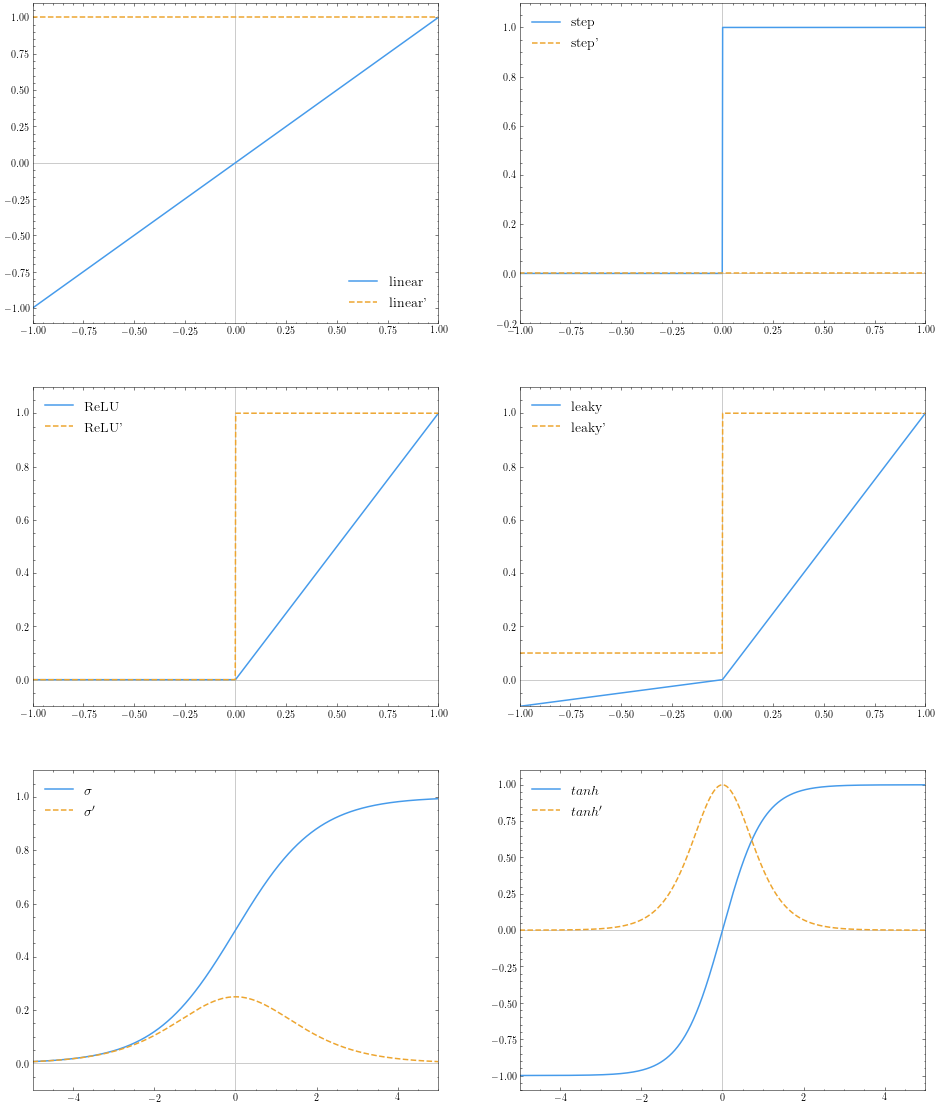
\includegraphics[width=15cm]{images/state-of-art/activation-functions/activation_functions.png}
    \caption{Gráficas de las funciones de activación}
    \label{fig:basicneuron}
\end{figure}

Cada neurona podría tener una función de activación asociada, pero por convención se usa un único tipo de función de activación por cada capa. Ambas soluciones aportan resultados similares y ninguna aporta en principio mejoras significativas al resultado del modelo. La principal diferencia es la complejidad que se añade a la hora de desarrollar una red si se quiere usar una función de activación distinta por neurona. En conclusión, siempre se opta por el uso de una única función de activación en todas las neuronas de una capa por simplicidad de desarrollo. 
\newline